\section{Sistema Mecânico}
Um sistema mecânico é constituído de quatro segmentos, todos com comprimento L, unidos entre si e a uma parede por articulações, vide a Figura~\ref{img:2}.
O momento em cada articulação é proporcional à deflexão com constante de proporcionalidade $\kappa$.
Os segmentos são feitos de material homogêneo de peso $P$.
A condição de equilíbrio pode ser expressa em termos dos ângulos $\theta_1,~\theta_2,~\theta_3,~\theta_4$ conforme à Equação~\ref{eq:2}.


\begin{equation}
\label{eq:2}
\begin{split}
    \kappa(\theta_1) 
     & = \frac{7PL}{2}  \cos(\theta_1) + \kappa(\theta_2 - \theta_1),
    \\ 
    \kappa(\theta_2 - \theta_1) 
    & = \frac{5PL}{2}  \cos(\theta_2) + \kappa(\theta_3 - \theta_2),
    \\ 
    \kappa(\theta_3 - \theta_2) 
    & = \frac{3PL}{2}  \cos(\theta_3) + \kappa(\theta_4 - \theta_3),
    \\ 
    \kappa(\theta_4 - \theta_3) 
    & =  \frac{1PL}{2} \cos(\theta_4)
\end{split}    
\end{equation}


Onde, $P = 15N,~ L = 1m$ e $\kappa = 100Nm/rad$.

\begin{figure}[!htp]
    \centering
    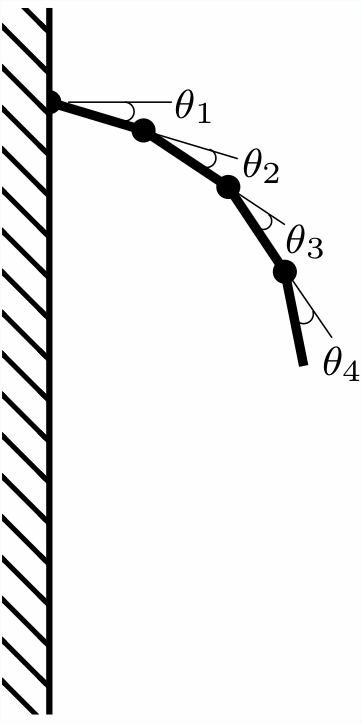
\includegraphics[scale=.2]{img/2.png}
    \caption{Sistema mecânico}
    \label{img:2}
\end{figure}







